\documentclass[a4paper,12pt,czech,bibliography=totoc]{scrbook}
\usepackage{ifthen}

\newboolean{compact}
\newboolean{feminum}

% odpoznámkujte, chcete li kompaktnější podobu textu (=méně stránek)  
%\setboolean{compact}{true}

% odpoznámkujte, jste-li žena (bude použit ženský rod v příčestích)
%\setboolean{feminum}{true}

\usepackage{amsmath,amssymb}

\usepackage{ifxetex}
\ifxetex
	%if xelatex
	\usepackage{fontspec}
	\setmainfont{Linux Libertine O}
	\setsansfont{Linux Biolinum O}
	\usepackage{unicode-math}
	\usepackage{polyglossia}
	\setdefaultlanguage{czech}
\else
	\usepackage[utf8]{inputenc}
	\usepackage[T1]{fontenc}
	\usepackage{libertine}
	\usepackage{fourier}
	\renewcommand{\ttdefault}{pxtt}
	\usepackage{babel}
\fi
\usepackage{graphicx}
\usepackage{graphics}
\usepackage{color}
\usepackage{listings}
\graphicspath{{images/}}

\lstset{ %
  language=C,                % the language of the code
  basicstyle=\small\ttfamily,    
  backgroundcolor=\color{white},   % choose the background color. You must add \usepackage{color}
  showspaces=false,                % show spaces adding particular underscores
  showstringspaces=true,           % underline spaces within strings
  showtabs=false,                  % show tabs within strings adding particular underscores
  frame=single,                    % adds a frame around the code
  tabsize=3,                       % sets default tabsize to 2 spaces
  breaklines=true,                 % sets automatic line breaking
  breakatwhitespace=false,         % sets if automatic breaks should only happen at whitespace
  keywordstyle=\bfseries,          % keyword style
  commentstyle=\rmfamily,       % comment style
  stringstyle=\itshape\color,   % string literal style
}

\usepackage{array}

\ifthenelse{\boolean{compact}}{
\usepackage[margin=2cm,includefoot,bindingoffset=0.5cm]{geometry}
}
{
\usepackage[margin=2.3cm,includefoot,bindingoffset=0.5cm]{geometry}
}
\usepackage{fancyhdr}

\fancyhf{}
\fancyfoot[CE,CO]{\arabic{page}}
\fancyhead[LE,RO]{\leftmark}
\fancyhead[LO,RE]{}

\fancypagestyle{plain}{%
\fancyhf{} % clear all header and footer fields
\fancyfoot[C]{\thepage} % except the center
\renewcommand{\headrulewidth}{0pt}
\renewcommand{\footrulewidth}{0pt}}

\pagestyle{fancy}

\renewcommand{\chaptermark}[1]{\markboth{\arabic{chapter}. #1}{}}

\ifthenelse{\boolean{compact}}{
\parindent=0pt % odsazení 1. řádku odstavce
\parskip=6pt   % mezera mezi odstavci
}{
\linespread {1.1}
\parindent=0pt % odsazení 1. řádku odstavce
\parskip=8pt   % mezera mezi odstavci
}

\newcommand{\UV}[1]{\quotedblbase{}#1\textquotedblleft{}}

\newcommand{\ZT}[1]{\colorbox{yellow}{\color{red}{#1}}}

\newcommand{\univerzita}{Univerzita Jana Evangelisty Purkyně \\v Ústí nad Labem}
\newcommand{\fakulta}{Přírodovědecká fakulta}
\newcommand{\katedra}{Katedra informatiky}
\newcommand{\obor}{Aplikovaná informatika}
\newcommand{\zamereni}{Informační systémy}
\newcommand{\nazevcz}{{Řízení domácnosti pomocí PLC a následná vizualizace pomocí webového serveru}}        % zde VYPLŇTE český název práce (přesně podle zadání!)
\newcommand{\nazeven}{{Controlling home via PLC and visualization using web server}}     % zde VYPLŇTE anglický název práce (přesně podle zadání!)
\newcommand{\autor}{{František Oplt}}           % zde VYPLŇTE své jméno a příjmení
\newcommand{\rok}{\the\year}                		% zde VYPLŇTE rok odevzdání, např. 2006
\newcommand{\vedouci}{{Ing. Petr Haberzettl}}         % zde VYPLŇTE jméno a příjmení vedoucího práce, včetně titulů
                                                               % např. Doc. Ing. Ivo Malý, Ph.D.
\newcommand{\pracovisteVed}{\katedra, \fakulta, \univerzita} % zde VYPLŇTE pracoviště vedoucího práce, je-li jiné než působiště

%\newcommand{\konzultant}{---} % POKUD MÁTE určeného konzultanta, NAPIŠTE jeho jméno a příjmení
%\newcommand{\pracovisteKonz}{} % POKUD MÁTE konzultanta, NAPIŠTE jeho pracoviště

\addto\captionsczech{%
  \renewcommand{\bibname}{Seznam použité literatury}%
}

\renewcommand{\arraystretch}{1.23}
\setcounter{secnumdepth}{2}
\setcounter{tocdepth}{1}

\usepackage{float}
\newfloat{algo}{htbp}{alg}[chapter]
\floatname{algo}{Algoritmus}
\definecolor{codegreen}{rgb}{0,0.6,0}
\definecolor{codegray}{rgb}{0.5,0.5,0.5}
\definecolor{codepurple}{rgb}{0.58,0,0.82}
\definecolor{backcolour}{rgb}{0.95,0.95,0.92}
\lstdefinestyle{mystyle}{
	backgroundcolor=\color{backcolour},   
	commentstyle=\color{codegreen},
	keywordstyle=\color{magenta},
	numberstyle=\tiny\color{codegray},
	stringstyle=\color{codepurple},
	basicstyle=\footnotesize,
	breakatwhitespace=false,         
	breaklines=true,                 
	captionpos=b,                    
	keepspaces=true,                 
	numbers=left,                    
	numbersep=5pt,                  
	showspaces=false,                
	showstringspaces=false,
	showtabs=false,                  
	tabsize=2
}

\lstset{style=mystyle}
\usepackage{algpseudocode}

\usepackage{varioref}
\usepackage{hyperref}

\begin{document}
\thispagestyle{empty}
\begin{center}
{
\LARGE
\univerzita\\[16pt]
\fakulta
}

\vspace{2cm}
\resizebox{4cm}{!}{
\includegraphics{prf-logo.png}}

\vspace{2cm}
{
\Huge\sffamily
\nazevcz\par
\Large\scshape bakalářská práce
}
\end{center} 
 
\vfill
{
\large
\begin{tabular}{>{\bfseries}rl}
    Vypracoval: 	& \autor\\
    Vedoucí práce: 	& \vedouci\\
&\\
Studijní program:       & \zamereni\\
Studijní obor:          & \obor\\
\end{tabular} 
}
\vspace{1.5cm}
\begin{center}
  \Large\scshape   Ústí nad Labem \rok
\end{center}

\cleardoublepage
\thispagestyle{empty}
\ZT{{\Huge zde vložte zadání!!!}}

\cleardoublepage

\thispagestyle{empty} 
{\bfseries Prohlášení} % SEM NESAHEJTE!

\vspace{0.5cm} % vertikální mezera. SEM NESAHEJTE!
Prohlašuji, že jsem tuto diplomovou/bakalárskou práci vypracoval\ifthenelse{\boolean{feminum}}{a}{}
samostatně a použil\ifthenelse{\boolean{feminum}}{a}{}
jen pramenů, které cituji a uvádím v přiloženém seznamu literatury.

\vspace{0.5em}

Byl\ifthenelse{\boolean{feminum}}{a}{} jsem seznámen\ifthenelse{\boolean{feminum}}{a}{} 
s tím, že se na moji práci vztahují práva a povinnosti vyplývající ze
zákona c. 121/2000 Sb., ve znění zákona c. 81/2005 Sb., autorský zákon, zejména se
skutečností, že Univerzita Jana Evangelisty Purkyně v Ústí nad Labem má právo na uzavření
licenční smlouvy o užití této práce jako školního díla podle § 60 odst. 1 autorského zákona, a
s tím, že pokud dojde k užití této práce mnou nebo bude poskytnuta licence o užití jinému
subjektu, je Univerzita Jana Evangelisty Purkyně v Ústí nad Labem oprávněna ode mne
požadovat přimerěný příspěvek na úhradu nákladu, které na vytvoření díla vynaložila, a to
podle okolností až do jejich skutečné výše.

\vspace{2em}

V Ústí nad Labem dne \today   \hfill Podpis: \makebox[3cm][s]{\dotfill}

\cleardoublepage
\thispagestyle{empty}
~
\vfill

\begin{flushright}
    Děkuji vedoucímu práce Ing. Petru Haberzettlovi \\ 
    za neocenitelné rady a pomoc při tvorbě bakalářské práce.
\end{flushright}

\cleardoublepage

\textsc{\nazevcz}

\textbf{Abstrakt:}

Bakalářská práce se zaměřuje na možnosti ovládání domácnosti pomocí webového rozhraní. Řízení domácnosti je realizováno pomocí programovatelného logického automatu (PLC). Jako PLC je použit nejnovější kontrolér od firmy Siemens, a to SIMATIC s7-1200. Pro ovládání je použit webový server. Webový server je navržen tak, aby se dal snadno použít i pro komunikaci s jinými zařízeními zabývajícími se domácí automatizací. Vzhled webového serveru je navržen tak aby umožnoval snadné ovládání pomocí mobilního telefonu.

\textbf{Klíčová slova:} PLC, automatizace, webový server

\bigskip


\textsc{\nazeven}

\textbf{Abstract:}

The bachelor thesis focuses on the possibilities of controlling the household through the web interface. Household control is implemented using a programmable logic controller (PLC). As the PLC is use the latest Siemens controller SIMATIC s7-1200. For controlling household is used web server. The web server is designed to be easy to use for communicating with other home automation devices. The appearance of the web server is designed to allow easy control over your mobile phone.

\textbf{Keywords:} PLC, automation, web server  


\tableofcontents
\setcounter{chapter}{0}
\chapter{Úvod}
Ve své bakalářské práci se zabývám možností ovládání některých prvků v domácnosti jako je například osvětlení nebo vytápění pohodlně pomocí webového aplikace. Ze začátku jsem se vydal cestou vývoje vlastního řešení postaveném na technologii asp.net. To se postupem času ukázalo jako špatná cesta. Nakonec jsem zvolil již existující platformu, do které jsem doprogramoval potřebné věci.
\newline
První část práce se zabývá stručným popisem použitých technologií. Popisuje použité komunikační protokoly a seznamuje čtenáře s problematikou programovatelných automatů.  
\newline
Druhá část popisuje použitý webový server. Popisuje způsob, jakým byl vybrán hardware určený pro plynulý chod aplikace. Dále je zde popsán způsob výběru webového serveru pro vizualizaci domácnosti.  
\newline
Třetí část se zabývá návrhem celého systému. Je zde popsáno, co všechno a v jakém rozsahu bude moci být ovládáno přes web. Dále je zde popsána topologie sítě, způsob komunikace webového serveru s PLC a rozvrženo pořadí jednotlivých prací.
\newline
Čtvrtá část se pak zabývá implementací programu pro PLC a kódu pro webový server.
\newline
Poslední kapitola se zabývá testováním celého systému.
 

\chapter{Popis použitých technologií}
\section{Modbus}
MODBUS je komunikační protokol na úrovni aplikační vrstvy modelu ISO/OSI, který umožňuje komunikaci typu Master-Slave. Na sběrnici je jeden Master (v případě MODBUS TCP i více) a několik Slave zařízení. Master posíla dotazy na Slave ražízení a ty odpovídají. Matster bývá většinou řídící prvek například průmyslové PC nebo PLC. Slave bývájí většinou čidla, měřící přístroje nebo PLC. Jako přenosová média MODBUS používá Ethernet (TCP/IP) nebo sériový přenos(RS-232, RS485, optické vlákno, atd.).
\subsection{Popis protokolu}
MODBUS definuje strukturu zprávy na úrovni protokolu(PDU - Protocol Data Unit) nezávislé na typu přenosového média. V závislosti na typu sítě je pak PDU rozšířena o další části a tvoří tak zprávu na aplikační úrovni (ADU - Application Data Unit)\\
Kód funkce udává zařízení typu slave (nebo Server) jakou operaci má provést. Rozsah je 0x01 až 0xff, přičemž kódy 0x80 až 0xff jsou vyhrazeny pro oznámení chyby.
\begin{figure}[h]
	\centering
	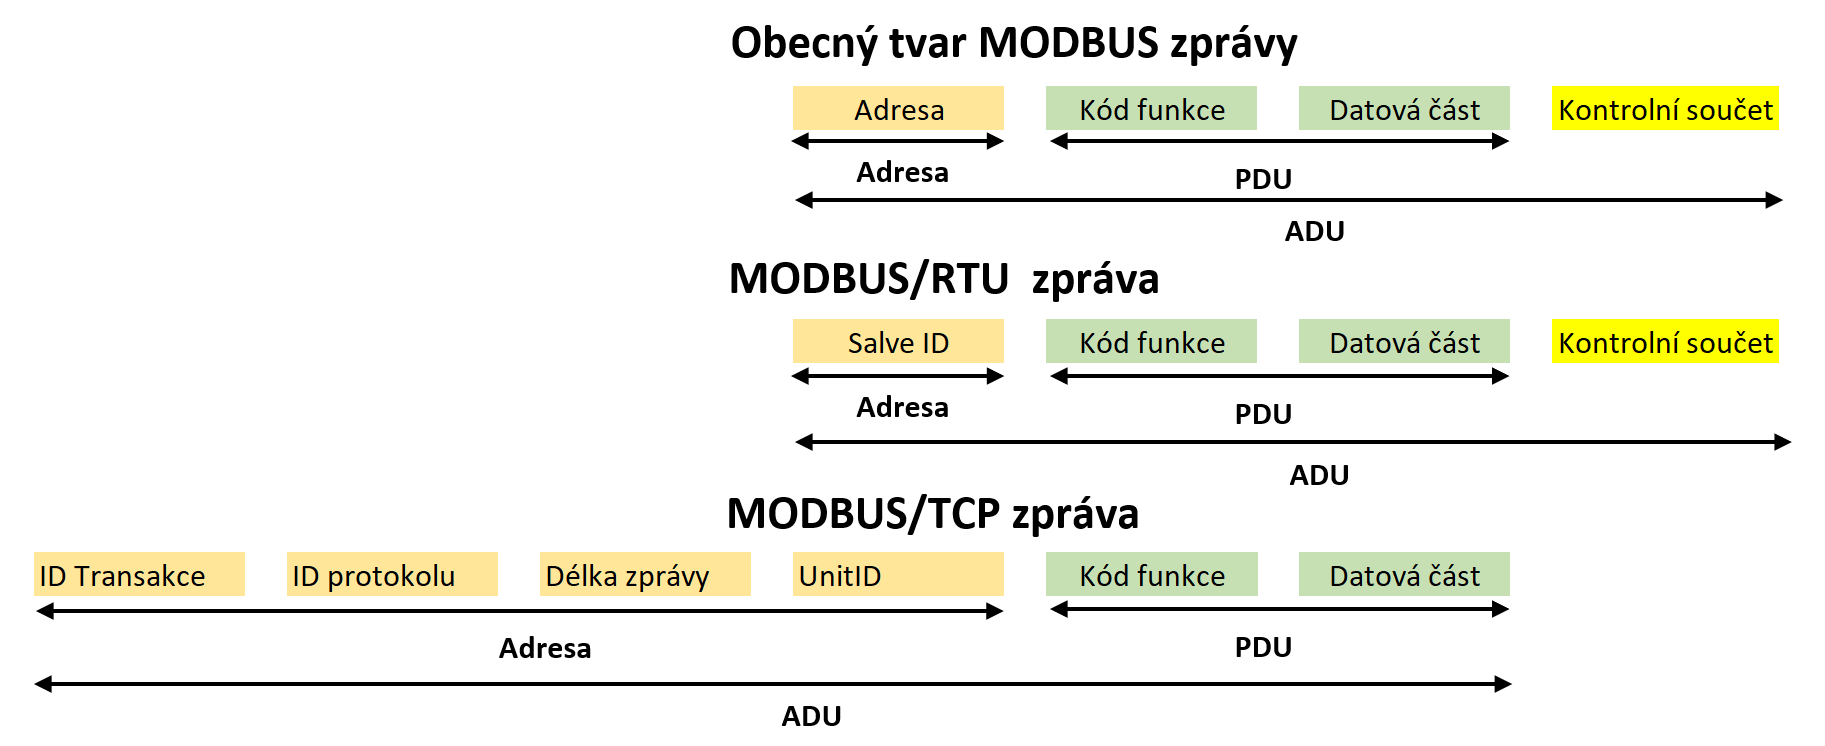
\includegraphics[scale=0.35]{modbus.PNG}
	\caption{Tvar modbus zprávy}
	\label{fig:my_label}
\end{figure}
\newpage
\subsection{Datový model}
Datový model je založen na tabulkách s charakteristickým významem. Jsou definovány čtyři základní tabulky Cívky, Diskrétní vstupy, Vstupní registry a Uchovávající registry. Mapování tabulek do adresního prostoru zařízení je závislá na konkrétním zařízení . Každá z tabulek může mít vlastní adresní prostor nebo se něj mohou dělit. Každá z tabulek může mít 65536 položek, ale z důvodu zpětné kompatibility bývá adresní prostor rozdělen na bloky o velikosti 10000 položek.
\begin{table}[h]
\centering
\begin{tabular}[h]{|c|c|c|c|c|}
	\hline
	\textbf{Tabulka} & \textbf{datový typ} & \textbf{Přístup} &\textbf{Adresa (SIMATIC)}\\
	\hline
	Cívky (\textit{Coils}) & bool & Čtení/Zápis & 1 až 9999\\  
	Diskrétní vstupy(\textit{Discrete Inputs}) & bool & Čtení & 10001 až 19999  \\
	Vstupní registry (\textit{Input Registers}) & WORD & Čtení & 30000 až 39999  \\
	Uchovávací registry (\textit{Holding Registers}) & WORD & Čtení/Zápis & 40001 až 49999 \\ \hline
\end{tabular}
\caption{Datový model protokolu Modbus}
\label{tab:my_label}
\end{table}
\section{Programovatelný automat (PLC)}
PLC (Programmable Logic Controller) neboli programovatelný logický automat je malý průmyslový počítač
přizpůsobený pro automatizaci procesů v reálném čase jako například montážní linky, robotické zařízení nebo
jakoukoliv činnost vyžadující vysokou spolehlivost, snadné programování a diagnostiku poruch procesu.
Hlavní rozdíl mezi PLC a klasickými počítači je ten že PLC jsou určena pro náročné podmínky (jako je prach,
vlhkost, chlad nebo teplo) a nabízí vstupy a výstupy (I/O) pro připojení senzorů a pohonů. Vstupy můžeme
mít analogové (snímaní teploty, tlaku, vlhkosti, ...) nebo binární (koncové snímače, tlačítka). Výstupy výstup
můžeme připojit např. sirény, elektromotory, solenoidy, relé nebo analogové výstupy.
\newline
\newline
 Program v PLC se provádí v cyklech. Na začátku každého cyklu se stav všech fyzických vstupů zkopíruje do oblasti paměti někdy nazývané "I/O Image Table", která je přístupná procesoru.  Procesor poté čte instrukce programu a provádí jednotlivé operace s daty. Po přečtení poslední instrukce procesor zpracuje požadavky z komunikací (modbus , s7), provede diagnostiku a aktualizuje výstupy. Délka celého procesu se nazývá scan time.
\cite{Berger2013}
\begin{figure}[h]
	\centering
	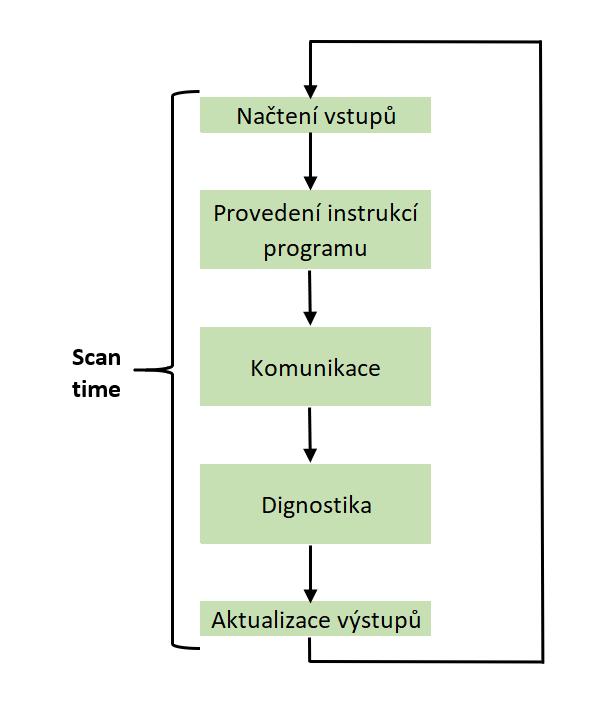
\includegraphics[scale = 0.6]{scanTime.PNG}
	\caption{Scan time}
	\label{fig:my_label}
\end{figure}
\subsection{SIMATIC S7-1200}
SIMATIC S7-1200 je modulární mikrokontrolér pro menší a střední automatizační úlohy. Kontroler se skládá z napájecího zdroje, samotné řídící jednotky a vstupně/výstupních modulů pro digitální a analogové signály. Toto PLC je vybaveno 1MB pamětí pro uživatelský program a 25KB operační paměti.
\newline
Paměťový prostor kontroleru je rozdělen na pět částí:
\begin{itemize}
	\item Process image input (I) - Na začátku každého cyklu je do této paměti zkopírován stav všech fyzických vstupů.\\
	\item Process image output (Q) - Na začátku každého cyklu je obsah této paměti zkopírován na fyzický výstup.\\
	\item Bit Memory (M) - Data zapsána do Bit memory jsou přístupná odkudkoliv z uživatelského programu. \\
	\item Temp memory (L) - Kdykoliv je zavolán některý blok kódu je mu přiřazena část této paměti.\\
	\item Data block (DB) - Paměť určená pro ukládání dat. \\
\end{itemize}
Pro programování kontroleru S7-1200 lze použít tři programovací jazyky LAD, FBD a SCL.
\cite{Stenerson2015}
\subsubsection*{LAD}
	LAD neboli ladder logika je vizuální programovací jazyk založený na konceptu reprezentace programu pomocí reléové logiky.  Program v jazyku LAD je zleva i zprava ohraničena svislými čarami, které reprezentují napájení. Mezi nimi je pak samotná logika programu.
	\begin{figure}[h]
		\centering
		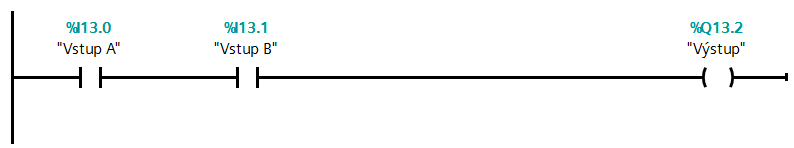
\includegraphics[scale = 0.6]{LAD_AND.PNG}
		\caption{Funkce AND zapsána pomocí jazyka LAD}
		\label{fig:my_label}
	\end{figure}
\subsubsection{FBD}
 FBD nebo-li Function Block Diagram je jazyk který popisuje program jako soubor vzájemně propojených grafických bloků obdobně jak je tomu u elektronických obvodovích diagramech. 
    	\begin{figure}[h]
    	\centering
    	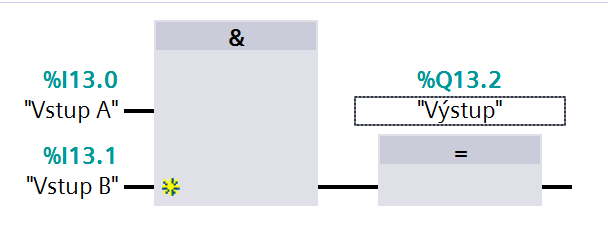
\includegraphics[scale = 0.6]{FBD_AND.PNG}
    	\caption{Funkce AND zapsána pomocí jazyka FBD}
    	\label{fig:my_label}
    \end{figure}
\subsubsection{SCL}
SCL je jazyk vhodný pro programování složitých algoritmů a aritmetických funkcí nebo pro zpracová dat. SCL kombinuje prvky známé z vyšších programovacích jazyků jako jsou například cykly nebo větvení a prvků známích z jazyků typických pro PLC jako je například adresování vstupů a výstupů.
	\begin{figure}[h]
	\centering
	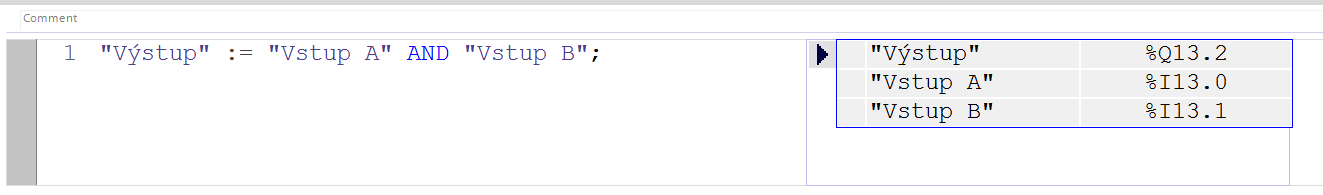
\includegraphics[scale = 0.5]{SCL_AND.PNG}
	\caption{Funkce AND zapsána pomocí jazyka SCL}
	\label{fig:my_label}
\end{figure}

\section{Z-Wave}
Z-Wave je bezdrátová technologie vyvinutá pro inteligentní řešení ovládání domácnosti. Umožňuje komunikaci mezi elektronickými zařízeními v domácnosti, jejich vzdálenou kontrolu a ovládání. Pro ovládání Z-Wave zařízení je zapotřebí řídící jednotka tzv. Z-Wave Gateway. V současné době Z-Wave podporuje více než 1700 výrobků od více než 450 výrobců. V Evropě používá Z-Wave frekvenci 868.42 MHz. Maximální přenosová rychlost je 100 Kbit/s. Maximální vzdálenost mezi dvěma zařízeními je 100 metrů. Pokud zařízení nemá přímé spojení s řídící jednotku může komunikovat až přes 4 další z-wave zařízení která fungují jako z-wave repeater celková vzdálenost pro komunikace je maximálně 200 metrů.
\section{1-Wire}
Tato sběrnice byla navržena firmou Dallas Semiconductor. Umožnuje připojit zařízení k řídící jednotce pomocí dvou vodičů. Při komunikaci na sběrnici se využívá model Master-Slave kde master je pouze jeden a bývá to většinou mikroprocesor. Slave zařízení může být na sběrnici připojeno více. Pro zapojení 1-wire zařízení se většinou používají tři vodiče. Napájecí vodič, datový vodič a zem. Datový vodič je spojen s napájecím vodičem pomocí 5kΩ odporu. 
\newline
Komunikaci zahajuje vždy master a to tak, že datový vodič uzemní (to způsobí že se na vodiči objeví logická 0) a v tomto stavu ho drží minimálně 480 mikrosekund. Poté datový vodič uvolní a naslouchá. Díky odporu se datový vodič vrátí do stavu log. 1. Pokud je na sběrnici připojeno nějaké zařízení tak tuto změnu detekuje a uvede datový vodič po dobu 60-240 mikrosekund do stavu log. 0 a tím se ohlásí řídící jednotce. Pokud se zařízení ohlásí tak master může vysílat nebo přijímat data.
\newline
Data jsou posílána v časových intervalech dlouhých 60 mikrosekund. V každém intervalu je poslán jeden bit. Pokud chce master poslat log. 1 tak na 1 – 15 mikrosekund vyšle na datový vodič log. 0 a zbytek intervalu ponechá log. 1.  Posílání log. 0 probíhá tak že master pošle na datový vodič log.0 a ponechá ji tam po celý interval.
\newline
Čtení probíhá tak, že master vyšle na datový vodič log. 0 a to po dobu 1 mikrosekundy. Poté může zařízení buďto vysílat log. 1 nebo log. 0.
\newline
Každé 1-wire zařízení obsahuje unikátní 64bitový identifikační kód. Pokud máme na síti více zařízení, musí se před posláním dat nejprve poslat adresa zařízení, pro které jsou data určena. 
\section{ESP8266}
ESP8266 je označení pro řadu mikropočítačů vyráběných společností Espressif Systém. Série ESP8266 v současné době obsahuje dva čipy ESP8266EX a ESP8285.
\newline
ESP8266EX je Soc, který integruje 32bitový mikroprocesor Tensilica, standartní digitální rozhraní (digitální vstupní a výstupní piny, různé typy sběrnic), anténu a modul pro řízení spotřeby. Obsahuje 2,4 GHz WiFi s podporou standardů 802.11 b/g/n.
 \newline
ESP8285 je variantou ESP8266 s 1024 KB Flash pamětí.
 \newline
Při použití ESP8266 máme k dispozici 32bit mikroprocesor s frekvencí 80 MHz 80 KB operační paměti. Dále je vybaven Flash pamětí pro ukládání programu. Velikost této paměti se pohybuje od 521 KB do 4 MB. Dále je k dispozici 16 Vstupně/výstupních pinů, SPI, I²C a UART sběrnice. 
\newline
Programovací jazyk pro vytváření programů pro EPS8266 je závislý na použitém firmwaru. Mezi nejpoužívanější firmware patří: NodeMCU (využívá jazyk LUA), Arduino (C++) a MicroPython.
\cite{Schwartz2016}


\section{MQTT}
MQTT je jednoduchý komunikační protokol určený pro internet věcí. Původně byl navržen firmou IBM, ale dnes již ve správě konsorcia Eclipse foundation. Protokol na předávání zpráv mezi klienty prostřednictvím centrálního serveru (tzv. broker). Server sbírá zprávy od poskytovatele zpráv (tzv. publisher) a předává je klientům které o ně mají zájem (tzv. subscribers). Jeden broker může mít libovolné množství poskytovatelů zpráv. Jakýkoliv klient může být jak Publisher, tak Subsriber. Publisher bývá snímač nebo měřící jednotka, která posílá naměřená data na server a subscriber tvoří řídící jednotka, která tyto hodnoty zpracovává.
\newline
\newline
Zprávy jsou rozděleny do témat (topic), přičemž každá zpráva patří právě do jednoto tématu. Témata jsou hierarchická a oddělená lomítky. Obsah zpráv není nijak definován, obsahem zprávy mohu tak být data libovolného formátu.  Velikost jedné zprávy je v současné době omezena na 256 MB.
\chapter{Specifikace a volba webového serveru}
Běh webového serveru zajišťuje jednodeskový počítač Raspberry Pi 3. Počítač je osazen čtyřjádrovým procesorem Broadcom BCM2837 s taktem 1.2 GHz a operační pamětí 1GB. Do počítačové sítě je připojen pomocí Ethernetu, který je integrován na desce počítače a podporuje maximální rychlost 100Mbit/s, která je v našem případě dostatečná. Důvodem pro výběr Raspberri Pi byla nízká cena, a především vysoká dostupnost.  \newline
U Raspberry pi 3 máme na výběr ze dvou operačních systému Windows 10 a Linux. Při testování se distribuce Windows 10 Iot určená speciálně pro Rasbberry Pi ukázala jako nevhodná, především kvůli vysoké nestabilitě. Byl tedy použit operační systém Raspbian. Jedná se oficiální Linuxovou distribuci pro Raspberry Pi.  
\section{Volba webového serveru}
PPři tvorbě webového serveru pro vizualizaci jsou na výběr celkem tři možnosti, jak postupovat:
\begin{itemize}
	\item Naprogramovat si vlastní webový server
	\item použít SCADA systém
	\item použít již existující platformu pro domácí automatizaci
\end{itemize}
Výhoda SCADy je v tom že je stavěná na propojení s PLC a má v sobě už všechny potřebné protokoly. SCADA systémy jsou učeny pro vizualizaci procesů v průmyslu, a z toho taky vyplývá jejich nevýhoda pro použití doma a to je vysoká cena.
\\
Nejideálněji řešení se nabízí použít už některou z vytvořených platforem pro domácí automatizaci. Taková to platforma by měla mít následující vlastnosti:
\begin{itemize}
	\item Responzivní vzhled
	\item snadná tvorba pluginů
	\item aktivní komunita
	\item kvalitní dokumentace
\end{itemize}
Výše zmíněným podmínkám vyhovují dvě platformy. Home Assistant a OpenHAB. 
Obě tyto platformy jsou rovnocenné. Nakonec byl zvolen Home Assistant a to z důvodu podpory více pluginů a rychlejšího vývoje. 
\section{Home Assistant}
Home Assistant je open-source platforma určená pro domácí automatizaci. Home assistant využívá programovací jazyk python3. Díky tomu může běžet na všech operačních systémech, které mají potporu pythonu3. Rozšířením pro Home Assistant se říká komponenty. V aktuální verzi (0.66.1) je k dispozici 1036 komponent. 
\cite{VCnCmsNRtY9uRcGa} 
	\subsection{Instalace}
	Pro instalaci nejnovější verze Home Assistantu je požadovýna minimální verze pythonu 3.5.3. Déle je doporučeno nainstalovat Home Assistant do virtuálního prostředí.
	\begin{itemize}
		\item Vytvoření virtuálního prostředí
			\begin{lstlisting}
			   $ python3 -m venv homeassistant
			\end{lstlisting}
		\item otevení vituálního prostředí
		 	\begin{lstlisting}
		     $ cd homeassistant
		  \end{lstlisting}
		\item Aktivace virtuálního prostředí
			\begin{lstlisting}
	   		$  source bin/activate
		  \end{lstlisting}
		\item instalace knihovny wheel
		\begin{lstlisting}
		  $ python3 -m pip install wheel
		\end{lstlisting}
		\item instalace Home Assistantu
			\begin{lstlisting}
	    	$ python3 -m pip install homeassistant
		\end{lstlisting}
		\item Spuštění
		\begin{lstlisting}
	    	$ hass
		\end{lstlisting}
	\end{itemize}
	\subsection{Konfigurace a přidávání komponent}
	Home Assistant ukládá konfiguraci do souboru s názvem \textit{configure.yaml}. Tento soubor se vygeneruje automaticky při prvním spuštění aplikace. Některé věci je možné upravovat přímo z uživatelského rozhraní, ostatní vyžadují ruční úpravu konfiguračního soubor. Pro editaci konfigurační souboru je dobré použít textový editor s podporou YAML syntaxe například Visual Studio Code nebo Atom.
	Pokud je třeba například přidat senzor, který bude generovat náhodné hodnoty, stačí do konfiguračního souboru přidat následují dva řádky:
		\begin{lstlisting}
	senzor:
	    platform: random
	\end{lstlisting}
	Seznam všech komponent a vzorové příklady jak je použít je k nalezení na officiálních stránkách Home Assistantu.
		
	\subsection{Psaní automatizací}
	Home Assistant nabízí tvorbu tzv. automatizací což je prvek který lze přirovnat například k tvorbě eventů ve vyšších programovacích jazycích.
	Automatice se skládají ze tří části: Trigger, Condition a Action.
	\cite{u93u76ihSFaMdU5g}
	\newline
	\textbf{Trigger} (česky spouštěč) popisuje událost, která pokud nastane tak dojde ke spuštění automatizace. Může se jednat například o osobu, která přijde domu. To je v Home Assistentu reprezentováno změnou stavu u dané osoby z „not\_home“ na „home“.
	\newline
	\textbf{Conditions} (česky podmínky) jsou volitelné testy, které mohou omezit automatizaci, aby fungovala jenom v konkrétním případě. Například budeme chtít reagovat, pouze pokud je po západu slunce.
	\newline
	Třetí a poslední částí je \textbf{Action} (česky akce). Zde se definuje akce, která se provede při spuštění triggeru a zároveň splnění všech doplňujících podmínek. Může se jednat například o změnu teploty na termostatu.
	\newline
	Níže uvedený kód je příklad zápisu automatizace, která pokud osoba přijde domu po západu slunce tak rozsvítí světla. Pro detekci je zde použita komponenta device\_tracker, která sleduje zařízení připojená k WiFi.
	\newpage
	\begin{lstlisting}
		automation:
			alias: Zapni svetla kdyz prijdu domu
			trigger:
				platforn: state
					entity_id = device_tracker.frantisek_mobil
					from: 'not_home'
					to: 'home'
			condition:
				condition: sun
				event: sunset
				offset: "-1:00:00"
			action:
				service: light.turn_on
	\end{lstlisting}
	\subsection{Psaní scriptů}
	Scripty jsou sekvence akcí, které Home Assistant vykoná. Po vytvoření je script k dispozici jako samostatná entita, ale může být také vložený do automatizací. Stejně jako automatizace se i scripty píší ve značkovacím jazyce YAML. Základní struktura scriptů je seznam klíčů a k nim přiřazených hodnot, které obsahují jednotlivé akce.
	\newline
	Níže je příklad scriptu, který svém zavolání zapne světla v koupelně a poté pošle upozornění s textem „Světla v koupelně byla rozsvícena“. Pokud script obsahuje pouze jednu akci tak můžeme element „sequence“ vynechat.
	\cite{HA_Scripts}
		\begin{lstlisting}
Script:
	Muj_prvni_script:
		Sequence:
			- Service: light.turn_on
			  Data:
				  Entity_id: light.svetla_koupelna
			- Service: notify.notify
			  Data:
				  Message: "Svetla v koupelne byla rozsvicena“ 
	\end{lstlisting}
	
	\subsection{Tvorba vlastních rozšíření}	
		I když Home Assitant v základu obsahuje více než tisíc již vytvořených komponent, ne vždy tam najdeme to co potřebujeme. Proto není špatné se alespoň trochu seznámit s tvorbou vlastních komponent.  Každé rozšíření musí obsahovat objekt DOMAIN. V něm je uložen název komponenty a měl by se shodovat s názvem souboru. Dále soubor musí obsahovat metodu \textit{setup(hass, config)}. Tato metoda se volá pouze jednou a to při načtení komponenty. Jak už název napovídá uvnitř této metody se provádí inicializace našeho rozšíření. Množství parametrů metody setup se muže lišit v závislosti na typu rozšíření, ale parametry hass a config jsou přítomny vždy.
		\cite{HA_custom}
		\newline
		Základní objekty:
		\begin{itemize}
			\item \textit{hass} - tento objekt obsahuje instanci Home Assistantu
			\item \textit{hass.config} - v tomto objektu je uložena základní konfigurace Home Assistantu jako například umístění konfiguračního souboru
			\item \textit{hass.states} - objekt umožňující měnit stavi jednotlivých entit (např. světel) nebo sledovat jestli byli změněny
			\item \textit{hass.bus} - tento objekt umožňuje aktivovat nebo sledovat eventy
			\item \textit{hass.services} - v tomto objektu můžeme registrovat služby
		\end{itemize}
V níže uvedeném kódu je příklad komponenty, která reprezentuje teplotní čidlo.
\newpage
\begin{lstlisting}[language=Python]
from homeassistant.const import TEMP_CELSIUS
from homeassistant.helpers.entity import Entity
import random
DOMAIN = 'example'
#Inicializace platformy
def setup_platform(hass, config, add_devices, discovery_info=None):

	#Vytvoreni dvou instanci tridy ExampleSenzor (Vytvoreni dvou cidel)
	cidlo1 = ExampleSenzor()
	cidlo2 = ExampleSenzor()
	#objekt add_divice slouzi k registraci entit.
	add_devices([cidlo1 , cidlo2])
	
#Trida ExampleSensor reprezentuje entitu senzoru
class ExampleSensor(Entity):
		
	def __init__(self,name):
		#Inicializace senzoru.
		self._name = name
		self._state = None
	
	@property
	def name(self):
			#Tato metoda vraci nazev cidla
		return self._name

	@property
	def state(self):
		# Metoda vraci stav cidla. Napr. pokud se jedna o teplotni cidlo, tak vraci posledni namerenou hodnotu
		return self._state

	@property
	def unit_of_measurement(self):
		# Tato metoda vraci jednotky ve kterych cidlo provadi mereni. TEMP_CELSIUS je konstanta Home Assistantu
		return TEMP_CELSIUS

	def update(self):
		#Po zavolani teto metody dojde k aktualizaci merene hodnoty. Zaroven je to jedina metoda, ktera by mela ziskavat data pro Home Assistant
		self._state = random.randint(1,50)
\end{lstlisting}

\chapter{Návrh systému a způsob provedení}
\section{Popis provedení}
	V rámci této bakalářské práce bude realizována automatizace prvního patra rodiného domu. Všechna světla a některé zásuvky bude možné ovládat z webového rozhraní. Světla na wc a koupelně se budou automaticky po hodině vypínat.
	\newline
	 Na schodišti budou umístěna dvě difuzní čidla pro detekci pohybu, která budou zajišťovat automatické rozsvícení světel pokud bude zaznamenán pohyb. Světla na schodišti se automaticky po třiceti minutách vypnou.
	 \newline
	  V obývacím pokoji a na chodbě bude umístěno intimní osvětlení, které se každý večer ve stanovený čas zapne a druhý den ráno v určité době vypne. Bude zde také umístěno teplotní čidlo pro měření pokojové teploty.
	  \newline
	  Na radiátorech budou umístěny termostatické hlavice, které budou regulavat teplotu v místnosti.
\section{Topologie}
	Světla a zásuvky budou ovládané pomocí PLC. To se bude dát ovládat dvěma způsoby. První způsobem je pomocí webové rozhraní Home Asssistantu. Druhý způsob je ovládání pomocí spínačů umístěných na zdi. To nám zaručí, že v případě výpadku serveru bude možné pořád ovládat světla.
	\newline
	 Ovládání vytábění bude realizováno pomocí termostatických hlavic od firmy Danfoss. Ty budou komunikovat s řídící jednotkou Vera Plus pomocí technologie Z-Wave. Vera Plus bude sloužit jako gateway pro všechna Z-Wave zařízení. Komunikace mezi Home Assistantem a Vera Plus bude realizováno pomocí Ethernetu. Pro vyčítaní dat z Vera+ bude použito již hotové rozšíření pro Home Assistant.
	 \newline
	   Měření teploty realizováno pomocí čidel DS18B20, které komunikují pomocí sběrnice 1-Wire. Data z čidel budou vyčítána pomocí ESP8266 a dále posílaná do Home Assistantu pomocí protokolu MQTT.
\begin{figure}[h]
	\centering
	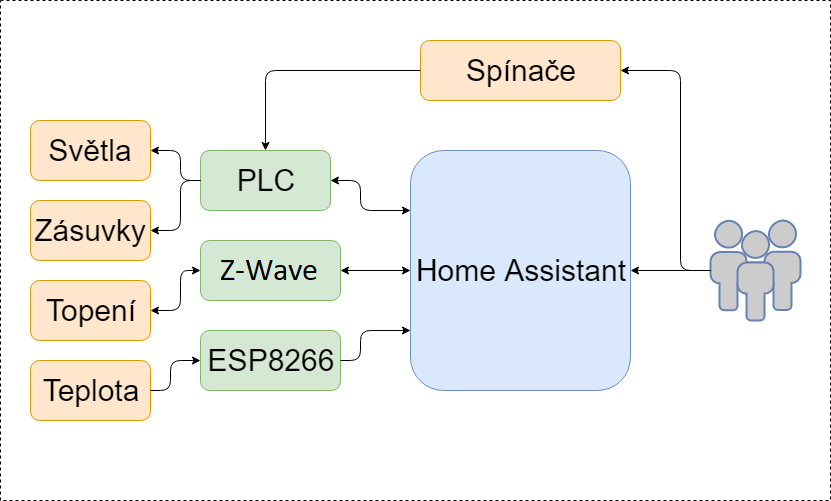
\includegraphics[scale = 0.5]{topologie.PNG}
	\caption{Topologie}
	\label{fig:my_label}
\end{figure}
\section{Pracovní postup}
Jako první je třeba připravit nový rozvaděč ve kterém bude umístěno PLC, napájecí obvody a jističe. Poté co bude nový rozvaděč na místě dojde k demontáži stávající elektroinstalace. V rámci nové elektroinstalace budou veškeré spínače a osvětlení svedeno do rozvaděče a napojeny na PLC. Jakmile bude elektroinstalace hotova bude vytvořen program pro PLC. Po dokončení PLC programu přijde na řadu instalace a konfiguraci Home Assistantu. Jakmile bude odladěna komunikace mezi PLC a Home Assistantem přijde na řadu zprovoznění vytápění.   
\section{Značení I/O}

	Digitální vstupy a výstupy jsou v PLC reprezentovány proměnou typu Bool a hardwarovou adresou. Adresa se skládá ze tří částí, první část tvoří písmeno, které nám říká jestli se jedná o vstup (I) nebo výstup (Q), následuje číslo Bytu v paměti a následně číslo bitu. Například I9.5 znamená že se jedná o digitální vstup, který najdeme v pátém bitu v devátém bajtu.
	\newline
	Analogové vstupy a výstupy jsou reprezentovány proměnou typu Word a jejich hardwarová adresa je ve tvaru IW10. První písmeno udává jestli se jedná o vstup (I) nebo výstup (Q), druhé písmeno nám říká že jde o Word tzn. Analogovou hodnotu a číslo označuje adresu v paměti kde je hodnota uložena.
	\newline	
	Před zahájením psaní programu je dobré si nejdříve vytvořit IO List, který bude obsahovat seznam všech vstupů a výstupů, datový typ, adresu a popřípadě komentář. Dále je dobré si stanovit metodiku pojmenování IO tak aby název každého IO byl v rámci programu unikátní a aby se z něj dalo na první pohled zjistit k čemu slouží.

\subsubsection{zvolená metodika}
\begin{figure}[h]
	\centering
	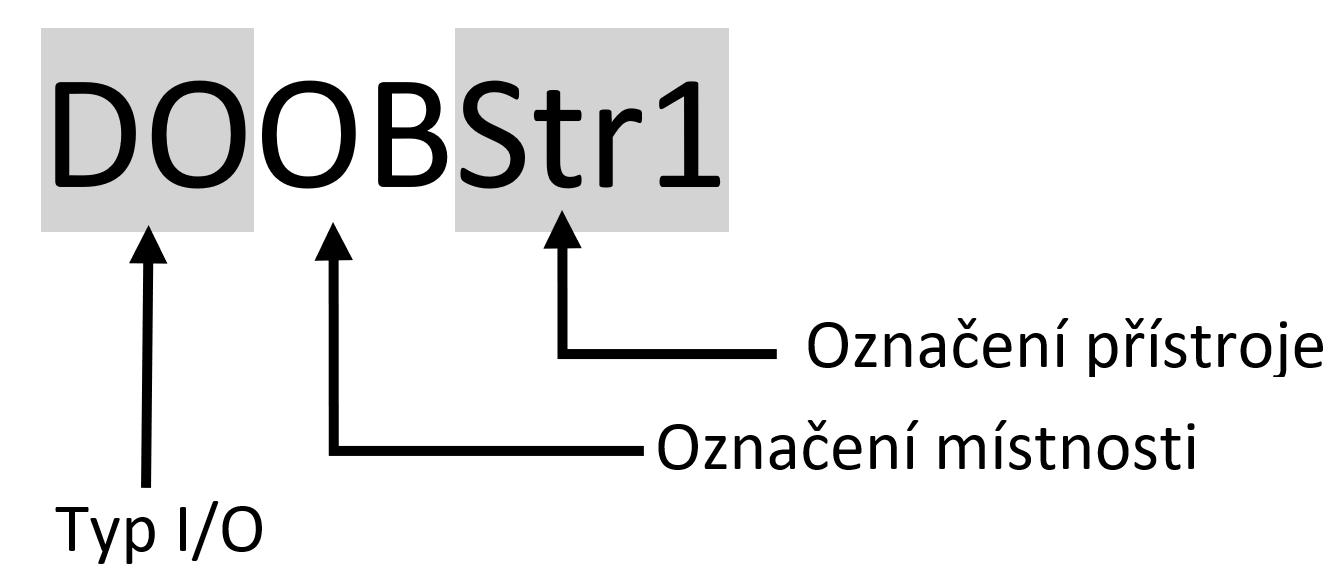
\includegraphics[scale = 0.3]{tagname.PNG}
	\caption{Značení přístojů}
	\label{fig:my_label}
\end{figure}

První dvě písmena v názvu určují typ I/O. Poté následují dvě písmena s onznačením místnosti. Počet posledních znaků není pevně stanoven, obsahuje minimálně tři písmena s označením přístroje a pokud je v místnosti více stejných přístrojů tak je zde ještě číslo přístroje.
	
\begin{table}
	\centering
\begin{tabular}[h]{|c|c||c|c|}
	\hline
    \textbf{zkratka} & \textbf{úplný název}&\textbf{zkratka} & \textbf{úplný název}	\\
	\hline
	DI & digitální vstup & Spi & Spínač\\	\hline
	DO & digitální výstup &Str & Stropní světlo\\	\hline
	AI & analogový vstup &Ste & Nástněnné osvětlení\\	\hline
	AO & analogový výstup &Led & LED osvětlení\\	\hline
	OB & Obývací pokoj & Cid & pohybové čidlo\\	\hline
	LO & Ložnice &Zas & Zásuvka\\	\hline
	PR & Pracovna& &\\	\hline
	KO & Koupelna & &\\	\hline
	WC & Záchod & &\\	\hline
	BA & Balkón	& &\\	\hline	  
\end{tabular}
\caption{Seznam zkratek}
\label{tab:my_label}
\end{table}


\section{Přenos dat mezi PLC a serverem Home assistant}
Na výstupní svorky PLC máme připojeno celkem 28 zařízení. Všechna zařízení se ovládají pomocí binárních signálů, k ovládání každého zařízení nám tedy bude stačit pouze jeden bit. Velikost holding registru je 16 bitů. Pro přenos ovládání všech zařízení nám tedy budou stačit dva registry.
Přenos dat z PLC do Home assistantu bude obstarávat protokol Modbus TCP. PLC bude sloužit jako Modbus server a Home assistant jako klient. Aby PLC mohlo fungovat jako Modbus server stačí použít už připravený bloček MB\_SERVER, který je součástí standartní knihovny v prostředí TIA PORTAL V14. Po vložení stačí pouze nastavit potřebné parametry.
\newline
Na straně Home assistantu je situace komplikovanější. Home assistant sice obsahuje rozšíření pro práci s protokolem Modbus, to však umí do jednoho holding registru zapsat pouze informaci o stavu jednoho zařízení. Při použití tohoto rozšíření bychom tedy potřebovali 28 registrů. Takové množství dat by způsobilo viditelné zpomalení celého programu.
\subsection{Návrh modbus rozšíření pro Home Assistant}
Rozšíření je složeno ze dvou soborů \textit{plc\_modbus.py} a \textit{modbus\_sw.py}. 
\newline
\subsubsection{plc\_modbus.py}
Tento soubor obsahuje vše potřebné pro komunikaci s PLC pomocí protokolu ModbusTCP. Pro komunikaci je použita knihovna \textit{pymodbus}. 
\newline
\textbf{setup\_platform} - rozšíření bude poskytovat Home Assistentu dvě služby. Službu \textit{handle\_write} po jejímž zavolaní boudou do PLC zapsány všechny registry ve kterých došlo ke změně hodnoty registru. Dále bude poskytovat službu \textit{handle\_read}, která má za úkol získat skutečný stav registrů uložených v PLC.
\newline
\newline
\textbf{RegisterHandler} - Třída představuje jeden register. Tato třída nekomunikuje s PLC přímo, ale využívá při tom metody třídy \textit{Communication}
  \begin{itemize}
  	\item \textbf{register\_number} - v tomto objektu je uloženo číslo registru v PLC, kterému tento registr odpovídá.
  	\item \textbf{ip} - Ip adresa PLC ve kterém je registr uložen.
  	\item \textbf{port} - Port přes který se má komunikovat s PLC (V PLC je pro každý registr vyhrazen jeden port, aby mohla komunikace probíhat paralelně).
  	\item \textbf{reg\_value }- 16bitová hodnota která představuje číselnou hodnotu registru.
  	\item \textbf{status\_change} - Informace o tom jestli od poslední synchronizace s PLC došlo ke změně registru.
  	\item \textbf{write\_reg()} - Slouží pro zápis registru do PLC. Zápis probíhá pouze v případě, že proměná \textit(status\_value) má hodnotu \textit{True} (došlo ke změně v registru)
  	\item  \textbf{read\_reg()} - Metoda pro čtení dat z PLC. Díky této metodě je zajištštěno, že \textit{RegisterHandler} a příslušný registr v PLC budou mít stejnou hodnotu
  	\item \textbf{set\_bit()} - Pokud dojde ke stisku tlačítka na webovém rozhraní, tak tlačítko zavolá tuto metodu a ta změní hodnotu příslušného bitu v proměné \textit{reg\_value}
  	\item \textbf{status()} - Tato metoda vrací aktuální stav konkrétního bitu v proměnné \textit{reg\_val} 
  \end{itemize}
\textbf{Communication} - Tato třída má na starosti přenos dat mezi Home Assistantem a PLC. K přenosu dat využívá knihovnu \textit{pymodbus}. Třída obsahuje metodu \textit{write\_register} pro zápis hodnoty jednoho registru do PLC. A metodu \textit{read\_register} pro přečtení hodnoty jednoho registru z PLC. Pokud by v budoucnu došlo ke změně komunikačního protokolu. Napříkald z protokolu Modbus TCP na S7 tak stačí změna imlementace této třídy.
\subsubsection{modbus\_sw.py}
Soubor modbus\_sw.py obsahuje metody a třídy potřebné pro implementaci spínačů napojených na komunikaci Modbus TCP.
\newline
\textbf{setup\_platform} - Tato metoda se zavolá při spuštění Home Assistantu a má na starosti vytvoření tlačítek. Vytváří instace třídy \textit{RegisterHandler}. Každé instanci přidá ip adresu PLC, číslo registru a port. Dále přiřadí tlačítka k jednotlivým registrům.
\newline
\textbf{ModbusSwitch} - Tato třída reprezentuje jeden spínač. Obsahuje tyto metody:
\begin{itemize}
	\item \textbf{name} - Metoda vrací název tlačítka
	\item \textbf{is\_on} - Tato metoda vrací aktuální stav tlačítka
	\item \textbf{turn\_on} - Zapne tlačítko
	\item \textbf{turn\_off} - Vypne tlačítko
\end{itemize}

Pro synchronizaci dat slouží script \textit{script\_modbus\_update} tento script volá metody \textit{handle\_write} a \textit{handle\_read}.\\ Volání scriptu každou vteřinu zajištuje automatizace \textit{automation\_modbus\_update}  


\begin{figure}[h]
	\centering
	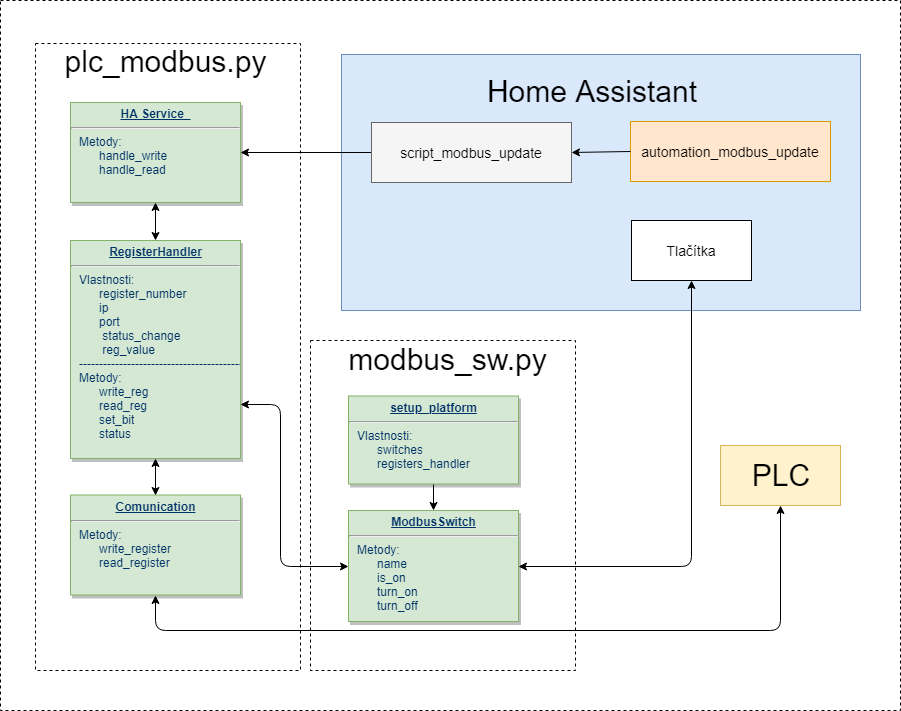
\includegraphics[scale = 0.5]{modbusDiagram.PNG}
	\caption{Modbus komunikace s HA}
	\label{fig:my_label}
\end{figure}



\chapter{Implementace}
\section{Ovládání výstupů}

	Jeden ze základních požadavků na systém je, aby se veškeré spotřebiče připojené k PLC dali ovládat jak místně tak pomocí webové stránky. V programu jsou pro tento problém implementovány dva bločky.
	\newline
	\subsection{TL1}
		První z nich TL1 slouží pro ovládání jednoho zařízení pomocí jednoho hardwarového vstupu a pomocí komunikace.
	\begin{figure}[h]
		\centering
		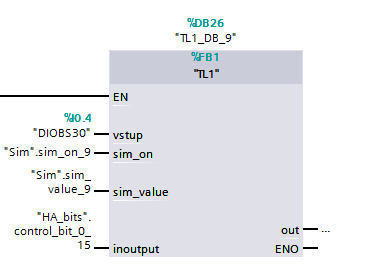
\includegraphics[scale = 1]{TL1.PNG}
		\caption{TL1}
		\label{fig:my_label}
	\end{figure}
\newline
Bloček umožňuje simulovat hardwarový vstup, to je užitečné zejména v případě že potřebujeme otestovat funkčnost ještě před tím, než připojíme hardwarový vstup, nebo pokud se vstup nachází na rozšiřující kartě, která z nějakého důvodu není k dispozici.
\newline
Výstupní signál můžeme připojit dvěma způsoby. Připojit hardwarový výstup přímo na výstup bločku (\textit{out}), nebo to udělat později v programu a použít k tomu proměnou která je přiřazená k \textit{inoutput}.
\subsubsection{Vnitřní impementace TL1}
Pro přehlednost je vnitřní struktura TL1 rozdělena na čtyři části.
V první části se hodnota z \textit{inoutput} přiřadí k proměnné \textit{pametBit}. 
\newline
Druhá část obsahuje implementaci režimu simulace. Pokud je \textit{sim\_on} nastaven na True tak se do proměnné \textit{vstup2} uloží hodnota \textit{sim\_value}. Pokud ne uloží se tam hodnota proměnné \textit{pamet}. První bloček z leva nám zajistí to, že se hardwarový vstup uloží do proměnné \textit{pamet}. Písmeno P znamená, že do proměnné \textit{pamet} se uloží True pouze tehdy mění-li se signál na hardwarovém vstupu z False na True (náběžnou hranu).
\begin{figure}[h]
	\centering
	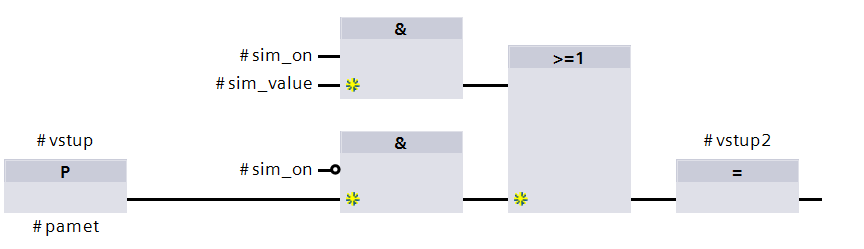
\includegraphics[scale = 0.8]{TL1_s2.PNG}
	\caption{TL1 simulace}
	\label{fig:my_label}
\end{figure}
Poslední část programu obsahuje logiku pro ovládání výstupu. Ta je realizována pomocí funkce XOR

\subsection{TL2}
Druhý bloček s názvem TL2 slouží k ovládání dvou zařízení pomocí jednoho tlačítka, ale zároveň umožnuje přes webové rozhraní ovládat každé zařízení zvlášť.
Od TL1 se liší tím, že vyžaduje dvě proměnné pro komunikaci s webovým serverem, a kromě dvou výstupů pro zařízení (out1 a out2) obsahuje ještě výstup act. Ten nabývá hodnoty True pokud je aktivní alespoň jeden z výstupů.
\newpage
\begin{figure}[h]
	\centering
	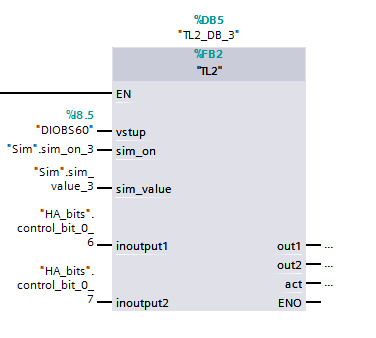
\includegraphics[scale = 1]{TL2.PNG}
	\caption{TL2}
	\label{fig:my_label}
\end{figure}
\subsubsection{Vnitřní impementace TL2}
Pro lepší přehlednost je program rozdělen na tři části. Z nichž první dvě jsou totožné s TL1.  třetí část, která obsahuje logiku se od logiky pro TL1 liší tím, že musí zajistit aby pokud je jeden z výstupů aktivní a dojde ke stisknutí tlačítka musí se oba výstupy nastavit na hodnotu False.
\begin{figure}[h]
	\centering
	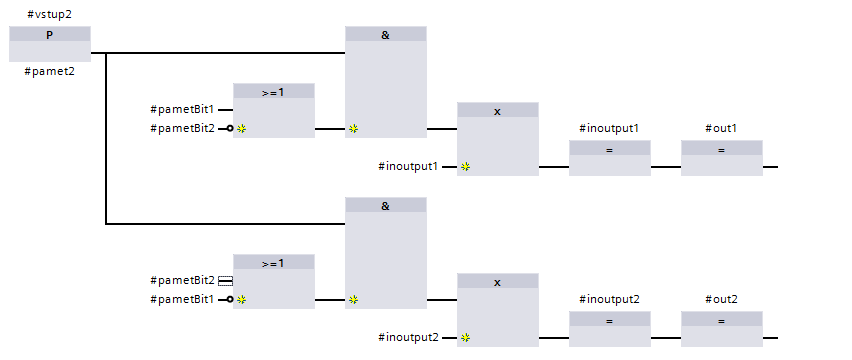
\includegraphics[scale = 0.6]{TL2_s3.PNG}
	\caption{TL2 logika}
	\label{fig:my_label}
\end{figure}
\section{Implementace Modbus rozšíření}
\subsection{RegisterHandler}
\begin{lstlisting}[language=Python]
class RegisterHandler:
	register_number = 0
	ip = "192.168.1.5"
	port = 502
	reg_value = 15
	change = False
	def __init__(self,register,ip,port):
		self.register_number = register
		self.ip = ip
		self.port = port
		self.reg_value = Comunication.readRegister(self.ip, self.port, self.register_number)

	def write_reg(self):
		if self.change:
			Comunication.writeRegister(self.ip, self.port, self.register_number, self.reg_value)
			self.change = False

	def status(self,index):
		mask = 1<<index # spocita masku
		value = mask & self.reg_value # zjisti hodnotu pozadovaného bitu
		if value == 0:
			return False
		else:
			return True

	def read_reg(self):
		if not self.change:
			self.reg_value = Comunication.readRegister(self.ip, self.port, self.register_number)

	def set_bit(self,index,x):
		mask = 1 << index  # Spocita masku
		self.reg_value &= ~mask  #  Smaze hodnotu požadovaného bitu
		if x:
			self.reg_value |= mask  # Pokud X = True tak nastavi požadovaný bit na 1
			self.change = True
\end{lstlisting}
\subsection{Comunication}
Tato třída implementuje kumunikaci s PLC pomocí protokolu Modbus TCP. Komunikace probíhá tak, že se naváže spojení s PLC. Poté se provede zápis/čtení registru do/z PLC. Po přenosu dat se spojení se PLC ukončí.
\begin{lstlisting}[language=Python]
	class Comunication:
		def writeRegister(ip, port,register, value):
			client = ModbusTcpClient(ip,port)
			client.write_register(register, value)
			client.close()
			return True

		def readRegister(ip, port,register):
			client = ModbusTcpClient(ip, port)
			result = client.read_holding_registers(register, 1)
			client.close()
			return result.getRegister(0)

\end{lstlisting}
\subsection{ModbusSwitch}
Implementace třídy \textit{ModbusSwitch} odpovídá svými metodami požadavkům na spínače, které jsou uvedeny v dokumentaci Home Assistantu. Pokud dojde ke stisknutí spínače zavolá se metoda \textit{turn\_on} popřípadě \textit{turn\_off}. Tyto metody změní příslušný bit ve svém registru. Každý spínač obsahuje odkaz na registr, ve kterém se nachází. \newpage
\begin{lstlisting}[language=Python]
class ModbusSwitch(SwitchDevice):

	def __init__(self, name, register,index):
		self._name = name
		self.register = register
		self.index = index
		self._state = False

	@property
	def name(self):
		return self._name

	@property
	def is_on(self):
		self._state = self.register.status(self.index)
		return self._state

	def turn_on(self):
		self.register.set_bit(self.index,1)
		self.is_on


	def turn_off(self):
		self.register.set_bit(self.index, 0)
		self.is_on
\end{lstlisting}

\subsection{Služby}
Při zavolání služby \textit{handle\_read} nebo \textit{handle\_write} dojde k postupnému zavolání metod \textit{write\_reg} nebo  \textit{read\_reg} u všech registrů.
\begin{lstlisting}[language=Python]
	def setup(hass, config):

		def handle_Write(call):
			for r in registers:
				r.write_reg()

		def handle_Read(call):
			for r in registers:
				r.read_reg()

hass.services.register(DOMAIN, 'plc_Write', handle_Write)
hass.services.register(DOMAIN, 'plc_Read', handle_Read)	
return True
\end{lstlisting}
\subsection{Inicializace}
Kromě standartních vstupních parametrů \textit{hass} a \textit{config} vstupuje do metody \textit{setup\_platform} ještě \textit{add\_device}. Tento objekt slouží k registraci nových zařízení. V poli \textit{switches} jsou uloženy všechny spínače.
\newline
První cyklus vygeneruje dva registry. Oba budou mít stejnou IP adresu (jsou umístěny na stejném PLC). Každý z registrů komunikuje s PLC na jiném portu. 
\newline
Ve druhém cyklu, se pro každý registr vytvoří 16 spínačů. Názvy spínačů jsou ve tvaru switch.x\_y. Kde \textit{x} představuje číslo registru a \textit{y} představuje číslo bitu. 

\begin{lstlisting}[language=Python]
	def setup_platform(hass, config, add_devices, discovery_info=None):
		registers = plcModbus.registers
		switches = []
		#simatic s7-1200 - prvni patro
		for i in range(0,2):
			r = plcModbus.RegisterHandler(i,"192.168.0.11", 502+i)
			registers.append(r)
			for spinac in range(0,16):
				# _LOGGER.info(a)
				switches.append(ModbusSwitch(str(i)+"_"+str(spinac),r,spinac))

		add_devices(switches)
\end{lstlisting}
\section{Konfigurace Home Assistantu}
	\subsection{skupiny}
	Home Assistant umožňuje sdružovat entity do skupin. Tyto skupiny se pak zobrazují na stejné kartě. V našem případě vytvoříme pro každou místnost samostatnou skupinu. Níže je ukázka, jak vypadají skupiny pro WC a koupelnu. 
	\begin{lstlisting}[language=Python]
	wc:
		name: Zachod
		entities:
			- switch.1_9

	koupelna:
		name: Koupelna
		entities:
			- switch.1_7
			- switch.1_8
	\end{lstlisting}

	\subsection{Úprava Entit}
	Protože entita s názvem \textit{switch.1\_9} nám sice řekne na kterém bitu a ve kterém registru se tlačítko nachází, ale pro každodenní používání to není příliš vhodné pojmenování. Naštěstí Home Assistant umožňuje ke každé entitě přiřadit název, který se bude zobrazovat na webovém rozhraní. Kromě názvu jde změnit i ikona. Například pro entitu, která ovládá světlo je dobré, aby se zobrazovala ikona žárovky.
		\begin{lstlisting}[language=Python]
switch.1_9:
	friendly_name: Svetlo
	icon: mdi:lightbulb-on-outline
	\end{lstlisting}
	\subsection{Konfigurační soubor}
Do konfiguračního souboru bylo přidáno několik komponent. Komponenta \textit{plc\_modbus} poskytuje služby pro komunikaci s PLC. Spínače, které jsou vygenerovány pomocí komponenty \textit{modbus\_sw} mají nastavený scan interval na dobu jedné sekundy. Díky tomu bude Home Assistant aktualizovat stav spínačů každou vteřinu. V aplikaci jsou použity tři druhy senzorů. První z nich využívá protokol MQTT pro vyčítání teploty v obývacím pokoji. Druhý slouží pro měření výkonu procesoru. To je zde především z důvodu testování, jestli Raspberri Pi 3 má dostatečný výkon pro Home Assistant. Třetí typ senzorů slouží pro měření aktuálního času.\\Komunikace se zařízením Vera+ je uskutečněno pomocí komponenty \textit{vera}, která dokáže automaticky detekovat a zobrazit všechna zařízení připojená k Vera Plus. Poslední přidaná komponenta je vstup pro zadávání času zapnutí/vypnutí intimního osvětlení.
\newpage
			\begin{lstlisting}[language=Python]
	plc_modbus:

	switch:
		- platform: modbus_sw
		  scan_interval: 1

	sensor:
	   - platform: mqtt
		   state_topic: "prvniPatro/obyvak/teplota"
	   - platform: systemmonitor
	    	resources:
	    	- type: processor_use
     - platform: time_date
		display_options:
		   - 'time'
		   - 'date'
		   - 'date_time'
		   - 'beat'
	vera:
		vera_controller_url: http://192.168.1.105:3480/

	input_datetime:
		chodba_od:
			name: Zapnuti svetel
			has_date: false
			has_time: true
	\end{lstlisting}
	
	\subsection{Změna vzhledu}
	Protože ne každému vyhovuje výchozí barévné schéma Home Assistantu, přidal jsem možnost měnit vzhled. Pro změnu vzhledu se používají předem připravená témata.
	\newline
	Pro vytváení témat slouží soubor \textit{themes.yaml}.
	\begin{figure}[h]
		\centering
		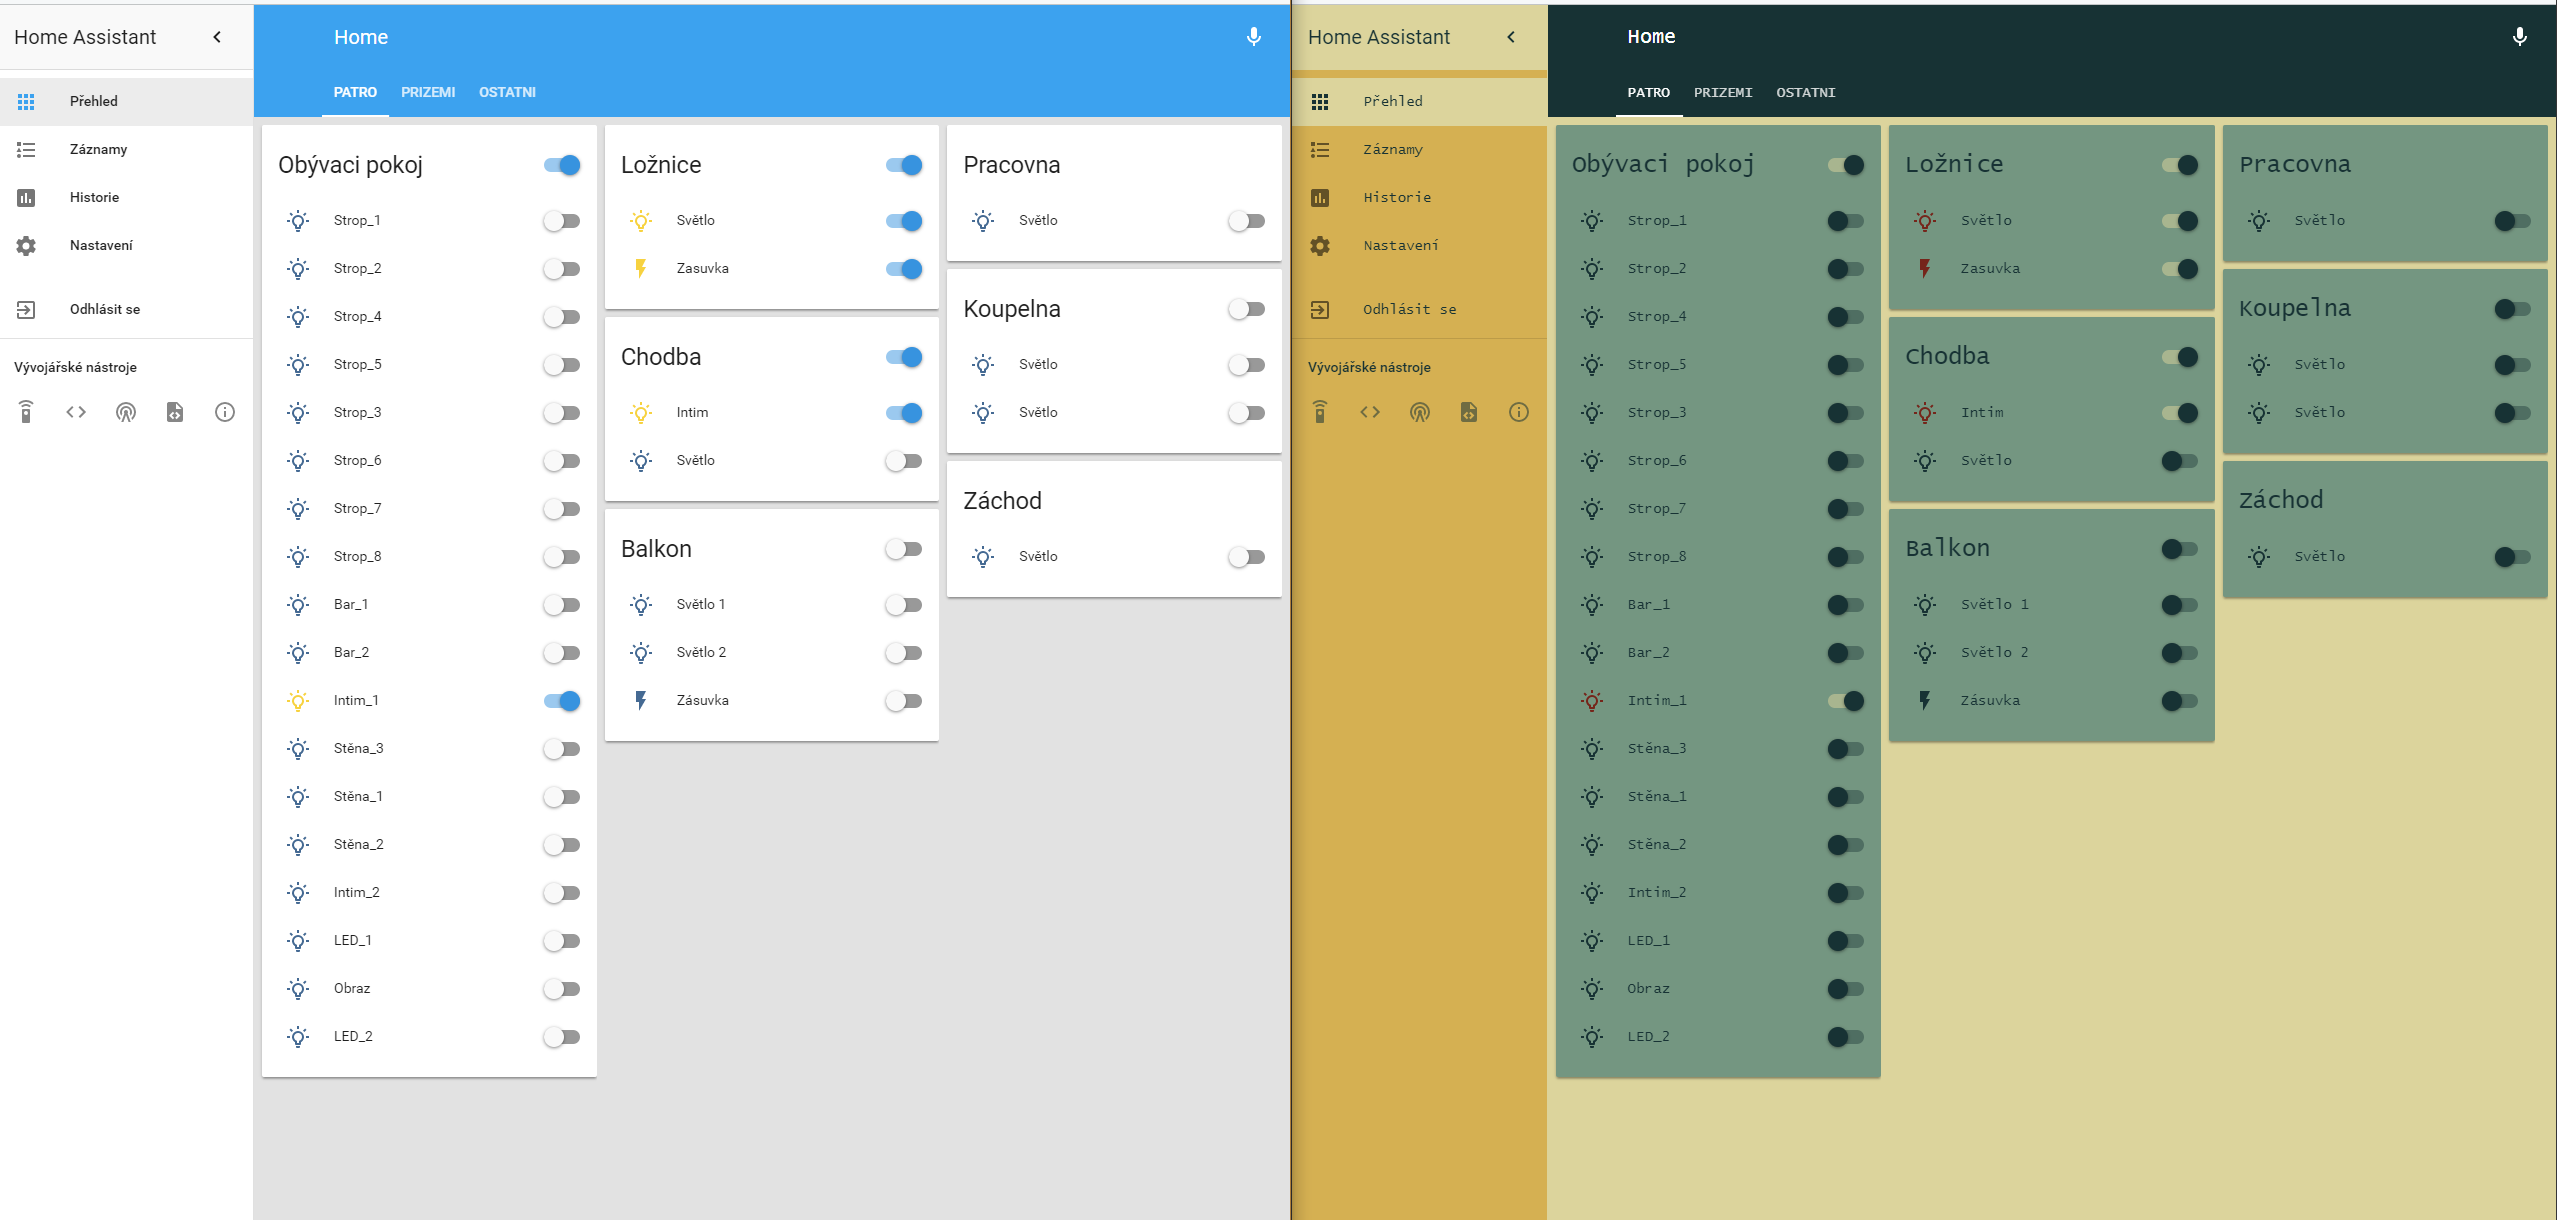
\includegraphics[scale = 0.2]{theme.PNG}
		\caption{Příklad změny vzhledu}
		\label{fig:my_label}
	\end{figure}
\section{Scripty a automatizace}
Pro vytváření Automatizací a Scriptů se mi osvědčilo používat editor integrovaný do webového rozhraní Home Assistantu. Jeho hlavní výhodou je, že se nemusí řešit syntaxe YAML. Díky tomu zvládne napsat jednoduché scripty nebo automatizace i člověk, který nemá s YAML žádné zkušenosti.
	\begin{figure}[h]
		\centering
		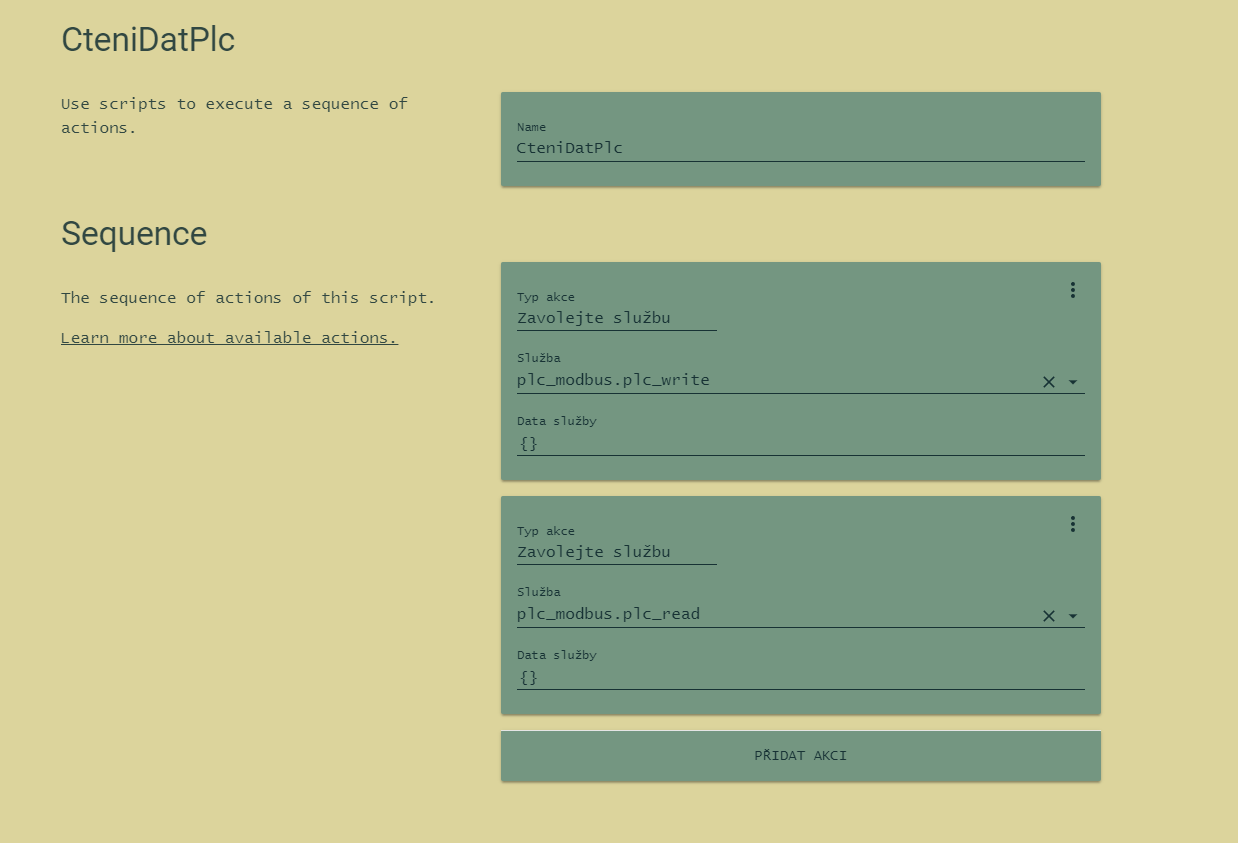
\includegraphics[scale = 0.3]{scriptEditor.PNG}
		\caption{Editor pro vytváření scriptů}
		\label{fig:my_label}
	\end{figure}
	\subsection{Intimní osvětlení}
	Automatizace na zapínání/vypínaní intimního osvětlení je řešena tak, že se porovnává aktuální systémový čas s časem zapnutí/vypnutí intimního osvětlení. Pokud se časy rovnají  zapne/vypne se příslušný spínač. 
	\newpage
		\begin{lstlisting}[language=Python]
- action:
	- alias: zapnuti_intim1_obyvak
	  data:
		entity_id: switch.0_10
	  service: switch.turn_on  
      condition: []
      id: '1522672482244'
      trigger:
      - platform: template
	  		value_template: '{{ states(''sensor.time'') == (states.input_datetime.obyvak_intim1_od.attributes.timestamp| int | timestamp_custom(''%H:%M'', False)) }}'

	\end{lstlisting}
	\subsection{Modbus}
	Synchronizace dat s PLC je realizováno pomocí scriptu \textit{CteniDatPlc}. Ten nejprve zavolá službu \textit{plc\_write}, která zapíše registry, ve kterých došlo ke změně. Poté co se dokončí zápis registrů do PLC, dojde k zavolání služby \textit{plc\_read}, která načte skutečný stav registrů.
\newline
O pravidelné spouštění scriptu se stará automatizace s názvem \textit{update\_modbus}. Jako trigger slouží systémový event \textit{time\_change}, který se vyvolá každou vteřinu. Dále je zde podmínka, aby automatizace běžela pouze pokud není spuštěn script \textit{CteniDatPlc}. Pokud je tato podmínka splněna tak se zavolá script pro aktualizaci registrů.

	\begin{lstlisting}
	alias: CteniDatPlc
	sequence:
		service: plc_modbus.plc_write
		service: plc_modbus.plc_read
	\end{lstlisting}
	\begin{lstlisting}
	- action:
		- service: script.1522670956418
	alias: update_modbus
	condition:
		- condition: state
		entity_id: script.1522670956418
		state: 'off'
	id: '1522671186544'
	trigger:
		- event_data: {}
		event_type: time_changed
		platform: event
	\end{lstlisting}
	\begin{figure}[h]
	\centering
	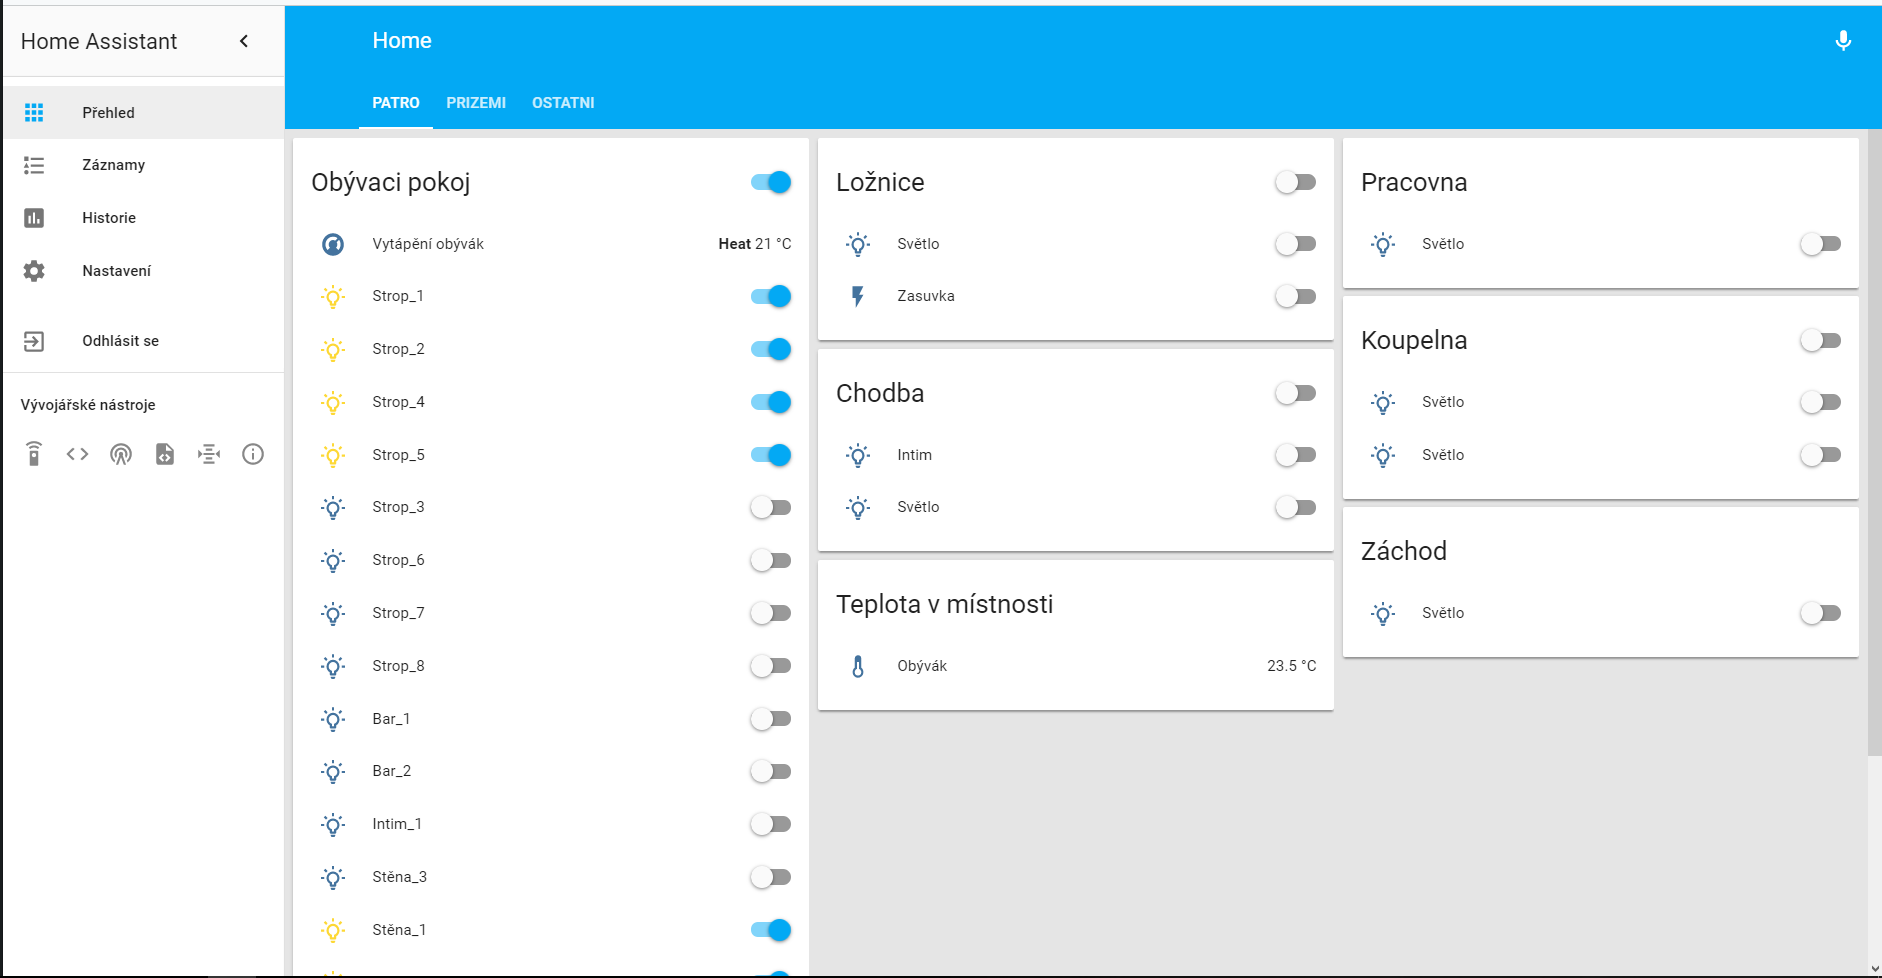
\includegraphics[scale = 0.3]{home.PNG}
	\caption{Home Assistant}
	\label{fig:my_label}
\end{figure}
\chapter{Ověření v praxi}
Testování bylo zahájeno 1. března 2018. Během testování se postupně zdokonaloval způsob komunikace s PLC. Jako první byla použita varianta, kde každý spínač funguje jako samostatná entita a o komunikaci s PLC se staral sám (neexistovala třída \text{RegisterHandler}). To se ukázalo jako velice nepraktické řešení, a to z toho důvodu, že doba od zmáčknutí spínače po rozsvícení příslušného světla trvali někdy i několik vteřin. 
\newline
Další z testovaných variant využívala buffer. Tento buffer představoval kopii jednoho PLC registru. Do tohoto bufferu byla automaticky každé dvě vteřiny uložena aktuální hodnota registru v PLC. O zápis do PLC se stále staral každý spínač sám. Tato verze už byla značně rychlejší. Především díky tomu, že o čtení dat už se nemusel start každý spínač samostatně. Místo toho bylo prováděno hromadně pro všechny spínače najednou. Nevýhodou tohoto řešení byl zápis. To se projevovalo zejména, když se uživatel pokusil vypnout více světel najednou. Kód byl v takovém případě nepředvídatelný. A tak ve výsledku se některá světla vypla a některá ne.
\newline
Nakonec byla použita varianta popsaná v kapitole 3.5.1. Která již netrpí žádným z nedostatků předchozích variant.
\newline
Během testovacího období nebyly zaznamenány žádné pády nebo jiné problémy, které by bránili používání Home Assistantu.


 
\chapter{Závěr}
Cílem této bakalářské práce bylo umožnit ovládání osvětlení, některých zásuvek a vytápění pomocí webového rozhraní. Tohoto cíle se jednoznačně dosáhnout povedlo. Celý systém se ukázal jako velice stabilní. A k dnešnímu datu (14.4.2018) nebyl zaznamenám, žádný problém, se stabilitou. Celý systém je navržen tak aby se dal snadno rozšířit. Díky tomu je možné přidat další místnosti nebo i celé patro s minimálními úpravami kódu. Ne vše se ale povedlo. Raspberry Pi se postupem času ukázalo jako špatná volba. I když výkonem zatím stačí, tak v případě přidání dalšího patra už nebude jeho výkon stačit. Bude tak potřeba zakoupit silnější počítač pro provozování Home Assistantu.
\newline
\newline
Veškeré zdrojové kódy, které v rámci této bakalářské práce vnikly jsou dostupné na přiloženém DVD. Z důvodu bezpečnosti byli z kódu odebrány veškeré historické záznamy a přístupové klíče. Kromě zdrojových kódů je k dispozici i krátké video s ukázkou funkčnosti. Pro zobrazení zdrojových kódů k PLC je potřeba TIA PORTAL V14 SP1 nebo vyšší.
\newline
\newline
S výsledkem bakalářské práce jsem velmi spokojen.


\begin{thebibliography}{99}	
\bibitem{Berger2013}
BERGER, Hans. \textit{Automating with SIMATIC S7-1200: configuring, programming and testing with STEP 7 Basic, visualization with HMI Basic}. 2., enl. and rev. ed. Erlangen: Publicis Publ, 2013. ISBN 9783895783852.
\bibitem{Stenerson2015}
STENERSON, Jon a David DEEG. \textit{Siemens Step 7 (Tia Portal) Programming, a Practical Approach}. 2015-07. Createspace Independent Publishing Platform, 2015. ISBN 9781515220541.
begin{thebibliography}{1}
\bibitem{Schwartz2016}
SCHWARTZ, Marco. \textit{Internet of Things with ESP8266} [online]. 1. Packt Publishing Limited, 2016 [cit. 2018-01-14]. ISBN 978-1786468024.
\bibitem{VCnCmsNRtY9uRcGa}
Home Assistant Components. \textit{Home Assistant} [online]. [cit. 2018-04-5]. Dostupné z: https://www.home-assistant.io/components/
\bibitem{u93u76ihSFaMdU5g}
Automating Home Assistant. \textit{Home Assistant} [online]. [cit. 2018-04-22]. Dostupné z: https://www.home-assistant.io/docs/automation/
\bibitem{HA_Scripts}
Script Syntax. Home Assistant [online]. [cit. 2018-04-22]. Dostupné z: https://www.home-assistant.io/docs/scripts/
\bibitem{HA_custom}
Creating components. \textit{Home Assistant} [online]. [cit. 2018-04-22]. Dostupné z: https://www.home-assistant.io/developers/creating\_components/
\bibitem{P0rotXtwgpP2s995}
Home Assitant Cookbook. \textit{Home Assitant} [online]. [cit. 2018-04-14]. Dostupné z: https://www.home-assistant.io/cookbook/
\bibitem{EizKg1TNj0hXRBul}
\textit{Home Assitant Development Guide} [online]. [cit. 2018-02-14]. Dostupné z: https://www.home-assistant.io/developers/
\bibitem{Gay2014}
GAY, Warren. \textit{Raspberry Pi hardware reference} [online]. New York, NY: Apress, 2014 [cit. 2018-04-14]. Technology in action series. ISBN 978-1-484208-00-7.
\end{thebibliography}

\listoffigures



\appendix

% \addpart{Přílohy} %pokud máte více příloh

\chapter{Obsah přiloženého CD}

\begin{tabular}{lp{8cm}}
  \hline
  soubor/adresář     &  obsah  \\
  \hline
  bakalarska\_prace.pdf   &   originální text diplomové práce \\
  Home\_Assistant/source\_code  & zdrojové kódy pro Home Assistant \\
  ESP8266/source\_code & zdrojové kódy pro ESP8266 (teploměr) \\
  PLC/source\_code & zdrojové kódy pro Simatic S7-1200 \\
  
  
\end{tabular}


\end{document}


